\documentclass[12pt]{report}
\usepackage{commands}

\begin{document}

\large
\begin{center}
AMSC 660 Homework 12\\
Due Dec 1\\
By Marvyn Bailly\\
\end{center}
\normalsize
\hrule

%Good luck my man
%---------------%
%---Problem 1---%
%---------------%


\begin{problem}%[vskip]
\subsection*{Problem 1}

Consider the KKT system 
\begin{equation*}
    \begin{pmatrix}
        G & A^\top\\ A & 0
    \end{pmatrix} \begin{pmatrix}
        -\mathbf{p} \\ \mathbf{\lambda}
    \end{pmatrix} = \begin{pmatrix}
        g \\ 0
    \end{pmatrix},
\end{equation*}
where $G$ is a $d\times d$ symmetric positive definite matrix and $A$ is $m\times d$ and has linearly independent rows. Show that the matrix
\begin{equation*}
    K := \begin{pmatrix}
        G & A^\top \\ A & 0
    \end{pmatrix}
\end{equation*}
is of saddle-point type, i.e., it has $d$ positive eigenvalues and $m$ negative ones.

\subsection*{Solution}
\begin{proof}

Consider the KKT system 
\begin{equation*}
    \begin{pmatrix}
        G & A^\top\\ A & 0
    \end{pmatrix} \begin{pmatrix}
        -\mathbf{p} \\ \mathbf{\lambda}
    \end{pmatrix} = \begin{pmatrix}
        g \\ 0
    \end{pmatrix},
\end{equation*}
where $G$ is a $d\times d$ symmetric positive definite matrix and $A$ is $m\times d$ and has linearly independent rows. Let's denote
\begin{equation*}
    K := \begin{pmatrix}
        G & A^\top \\ A & 0
    \end{pmatrix},
\end{equation*}
and consider the decomposition
\begin{equation*}
    \begin{pmatrix}
        G & A^\top \\ A & 0
    \end{pmatrix} = \begin{pmatrix}
        I & 0 \\ X & I
    \end{pmatrix} \begin{pmatrix}
        G & 0 \\ 0 & S
    \end{pmatrix}\begin{pmatrix}
        I & X^\top\\ 0 & I
    \end{pmatrix}.
\end{equation*}
Where we can find $G$ and $S$ by observing
\begin{align*}
    \begin{pmatrix}
        G & A^\top \\ A & 0
    \end{pmatrix} &= \begin{pmatrix}
        I & 0 \\ X & I
    \end{pmatrix} \begin{pmatrix}
        G & 0 \\ 0 & S
    \end{pmatrix}\begin{pmatrix}
        I & X^\top\\ 0 & I
    \end{pmatrix}\\
    &= \begin{pmatrix}
        G & 0 \\ XG & S
    \end{pmatrix} \begin{pmatrix}
        I & X^\top\\ 0 & I
    \end{pmatrix}\\
    &= \begin{pmatrix}
        G & GX^T \\ XG & XGX^\top + S
    \end{pmatrix}\\
    &= \begin{pmatrix}
        G & (XG)^T \\ XG & XGX^\top + S
    \end{pmatrix},
\end{align*}
and so $X = AG^{-1}$ as $G = G^\top$ since $G$ is SPD and we can solve for $S$ to get
\begin{align*}
    S = -XGX^\top = -AG^{-1}G(AG^{-1})^\top = -AG^{-1}A^{\top}.
\end{align*} 
Thus
\begin{equation*}
    \begin{pmatrix}
        G & A^\top \\ A & 0
    \end{pmatrix} = \begin{pmatrix}
        I & 0 \\ AG^{-1} & I
    \end{pmatrix} \begin{pmatrix}
        G & 0 \\ 0 & AG^{-1}A^{\top}
    \end{pmatrix}\begin{pmatrix}
        I & (AG^{-1})^\top\\ 0 & I
    \end{pmatrix},
\end{equation*}
Since $\begin{pmatrix}
    I & 0 \\ AG^{-1} & I
\end{pmatrix}$ and its transpose are nonsingular, we have that $K$ and $\begin{pmatrix}
    G & 0 \\ 0 & AG^{-1}A^{\top}
\end{pmatrix}$ are congruent. Then by Sylvester's law of inertia, $K$ and $\begin{pmatrix}
    G & 0 \\ 0 & AG^{-1}A^{\top}
\end{pmatrix}$ have the same number of positive, zero, and negative eigenvalues. Note that both matrices are size $d + m \times d + m$. Since $G$ is SPD and $d \times d$, it has $d$ real and positive eigenvalues. Next, let $(\lambda,v)$ be an eigenpair of $AG^{-1}A^{\top}$, observe that
\begin{align*}
    -AG^{-1}A^{\top} v &= \lambda v\\
    \Leftrightarrow -v^\top (AG^{-1}A^{\top}) v &= v^\top \lambda v\\
    \Leftrightarrow -(v^\top A) G^{-1} (v^{\top} A)^{\top} &= \lambda \|v\|^2
\end{align*}
Since $G$ is SPD, we have that $-(v^\top A) G^{-1} (v^{\top}A)^{\top} < 0$ where the strick inequality is since $A$ is of full rank and thus $v^\top A \neq 0, \forall v$. Furthermore, as $\|v\|^2 > 0$, we have that $\lambda < 0$. Thus $AG^{-1}A^{\top}$ has $m$ negative eigenvalues. Therefore, $\begin{pmatrix}
    G & 0 \\ 0 & AG^{-1}A^{\top}
\end{pmatrix}$ has $d$ positive eigenvalues and $m$ negative ones which gives that $K$ does as well. 





\end{proof}
\end{problem}




%---------------%
%---Problem 2---%
%---------------%


\begin{problem}%[vskip]
\subsection*{Problem 2}

Consider an equality-constrained quadratic problem QP 
\begin{align*}
    \frac{1}{2}x^\top G x + c^\top x &\rightarrow \min ~\text{subject to}\\
    Ax &= b.
\end{align*}
The matrix $G$ is symmetric. Assume that $A$ is full rank (i.e. its rows are linearly independent) and $Z^\top GZ$ is positive definite where $Z$ is a basis for the null-space of $A$, i.e., $AZ = 0$.
\begin{enumerate}
    \item [(a)]
    Write the KKT system for this case in the matrix form.
    \item [(b)]
    Show that the matrix of this system K is invertible. Hint: assume that there is a vector $z := (x, y)^\top$ such that $Kz = 0$. Consider the quadratic form $z^\top Kz$, use logical reasoning and algebra, and arrive at the conclusion that then $z = 0$.
    \item [(c)]
    Conclude that there exists a unique vector $(x^*, \lambda^*)^\top$ that solves the KKT system. Note that since we have only equality constraints, the positivity of $\lambda$ is irrelevant.
\end{enumerate}

\subsection*{Solution}
\begin{proof}

Consider an equality-constrained quadratic problem QP 
\begin{align}
    f(x) = \frac{1}{2}x^\top G x + c^\top x &\rightarrow \min ~\text{subject to}\\
    Ax &= b,
\end{align}
where $G$ is symmetric, $A$ is full rank, and $Z^\top GZ$ is positive definite where $Z$ is a basis for the null-space of $A$, i.e., $AZ = 0$.
\begin{enumerate}
    \item [(a)]
    To find the KKT system of this problem, let $x_k$ be the current iterate and consider the update 
    \begin{equation*}
        x_{k+1} = x_k + p_k.
    \end{equation*}
    Plugging this into Equation (1) yields
    \begin{align*}
        &\frac{1}{2}\paren{x_k + p_k}^\top G \paren{x_k + p_k} + c^\top \paren{x_k + p_k} =\\ 
        &= \frac{1}{2}p_k^\top G p_k + \paren{\frac{1}{2} x_k^\top G x_k + + c^\top x_k }+ \frac{1}{2} x_k^\top G p_k + \frac{1}{2}p_k^\top G x_k +  + c^\top p_k \\
        &= \frac{1}{2}p_k^\top G p_k + \paren{Gx_k + c}^\top p_k + f(x_k).
    \end{align*}
    Furthermore, notice that $G x_k + c = \nabla f(x_k)$ and since $f(x_k)$ is independent of $p_k$, it does not affect the minimizer. Next, we can plug $x_{k+1} = x_k + p_k$ into Equation (2) to get
    \begin{align*}
        A(x_k + p_k) - b = \paren{Ax_k - b} + A p_k = A p_k, 
    \end{align*}
    since $Ax_k - b = 0$. Therefore, the minimization problem for $p_k$ is of the form
    \begin{align*}
        \frac{1}{2}p^\top G p + \nabla f(x_k)^\top p &\rightarrow \min ~\text{subject to}\\
        Ap = 0.
    \end{align*}
    To find the KKT system, we compute the Lagrangian function of the problem to be
    \begin{equation*}
        L(p_k,\lambda) = \frac{1}{2}p_k^\top G p_k + \nabla f(x_k)^\top p_k - \lambda^\top(Ap_k).
    \end{equation*}
    Next, we compute the gradients to get
    \begin{equation*}
        \nabla_{p_k} L(p_k,\lambda) = G p_k + \nabla f(x_k) - A^\top \lambda \and \nabla_\lambda L(p_k,\lambda) = - Ap_k.
    \end{equation*}
    We can now rewrite the KKT system in matrix form as
    \begin{equation}\label{kkkktttt}
        \begin{pmatrix}
            G & A^\top\\ A & 0
        \end{pmatrix}\begin{pmatrix}
            -p_k \\ \lambda
        \end{pmatrix} = \begin{pmatrix}
            \nabla f(x_k) \\ 0
        \end{pmatrix}.
    \end{equation}
    
    
    
    \item [(b)]
    Now if we let
    \begin{equation*}
        K = \begin{pmatrix}
            G & A^\top\\ A & 0
        \end{pmatrix},
    \end{equation*}
    we wish to show that $k$ is nonsingular. To do so, assume that there exists $z := (x,y)^\top$ such that $Kz = 0$. Then we have that
    \begin{equation}\label{bigboisteve}
        \begin{pmatrix}
            G & A^\top\\ A & 0
        \end{pmatrix}\begin{pmatrix}
            x\\y
        \end{pmatrix} = 0,
    \end{equation}
    giving that $Ax = 0$. Thus we get that
    \begin{align*}
        0 &= \begin{pmatrix}
            x \\ y
        \end{pmatrix}^\top \begin{pmatrix}
            G & A^\top\\ A & 0
        \end{pmatrix} \begin{pmatrix}
            x \\ y
        \end{pmatrix} = x^\top G x + (Ax)^\top y + y^\top Ax = x^\top G x.
    \end{align*}
    Now since $x$ is in the null space of $A$, we can rewrite it as a $x = u Z$ for some vector $u$. This gives that 
    \begin{equation*}
        0 = x^\top G x = u^\top  \paren{Z^\top G Z} u, 
    \end{equation*}
    and since $Z^\top G Z$ is SPD, we have that $u = 0$ which gives $x = 0$. Furthermore, by plugging $x = 0$ into Equation \ref{bigboisteve}, we find that $A^\top y = 0$. Since $A$ is full row rank, $A^\top y = 0$ if and only if $y = 0$. Therefore $Kz = 0$ if and only if $z = 0$ which shows that $K$ is nonsingular.

    \item [(c)]
    Since $K$ is nonsingular, there exists a vector $v$ that satisfies \fullref{kkkktttt}, namely
    \begin{equation}
        v = \begin{pmatrix}
            x^*\\\lambda^*
        \end{pmatrix}= \begin{pmatrix}
            G & A^\top\\ A & 0
        \end{pmatrix}^{-1}\begin{pmatrix}
            \nabla f(x_k) \\ 0
        \end{pmatrix}.
    \end{equation}
    To show that $v$ is unique, assume there exists another vector $u$ such that $u \neq v$ and $u$ satisfies \fullref{kkkktttt}. Then we have that
    \begin{equation*}
        Kv = \begin{pmatrix}
            \nabla f(x_k) \\ 0
        \end{pmatrix} \and Ku = \begin{pmatrix}
            \nabla f(x_k) \\ 0
        \end{pmatrix}.
    \end{equation*}
    But this gives that
    \begin{equation*}
        Kv - Ku = K(v - u) = 0,
    \end{equation*}
    and since $u \neq v$, then $v - u \neq 0$ which contradicts $K$ being nonsingular. Therefore, there exists a unique vector $(x^*, \lambda^*)^\top$ which satisfies the KKT system \fullref{kkkktttt}. 
\end{enumerate}

\end{proof}
\end{problem}




%---------------%
%---Problem 3---%
%---------------%


\begin{problem}%[vskip]
\subsection*{Problem 3}

Consider the following quadratic program with inequality constraints:
\begin{flalign}
&   &f(x, y) = (x - 1)^2 + (y - 2.5)^2 \rightarrow \min & \quad \text{subject to} & &\\
& \text{[1]} & x - 2y + 2 &\geq 0 & & \\
& \text{[2]} & -x - 2y + 6 &\geq 0 & &\\
& \text{[3]} & -x + 2y + 2 &\geq 0 & &\\
& \text{[4]} & x &\geq 0 & &\\
& \text{[5]} & y &\geq 0 & 
\end{flalign}

\begin{enumerate}
    \item [(a)]
    Plot level sets of the objective function and the feasible set.

    \item [(b)]
    What is the exact solution to (6) - (11)? Find it analytically with the help of your figure.
    
    \item [(c)]
    Suppose the initial point is $(2,0)$. Initially, constraints $3$ and $5$ are active, hence start with $\mathcal{W} = \brac{3,5}$. Work out all iterations of the active-set method analytically. The arising linear systems should be very easy to solve. For each iteration, you need to write out the set $\mathcal{W}$, the KKT system, its solution, i.e., $(p_x,p_y)$, the vector of Lagrange Multipliers, and the current iterate $(x_k,y_k)$. Plot all iterations on your figure. There should be a total of $5$ iterations.

\end{enumerate}

\subsection*{Solution}
\begin{proof}

\begin{figure}
    \centering
    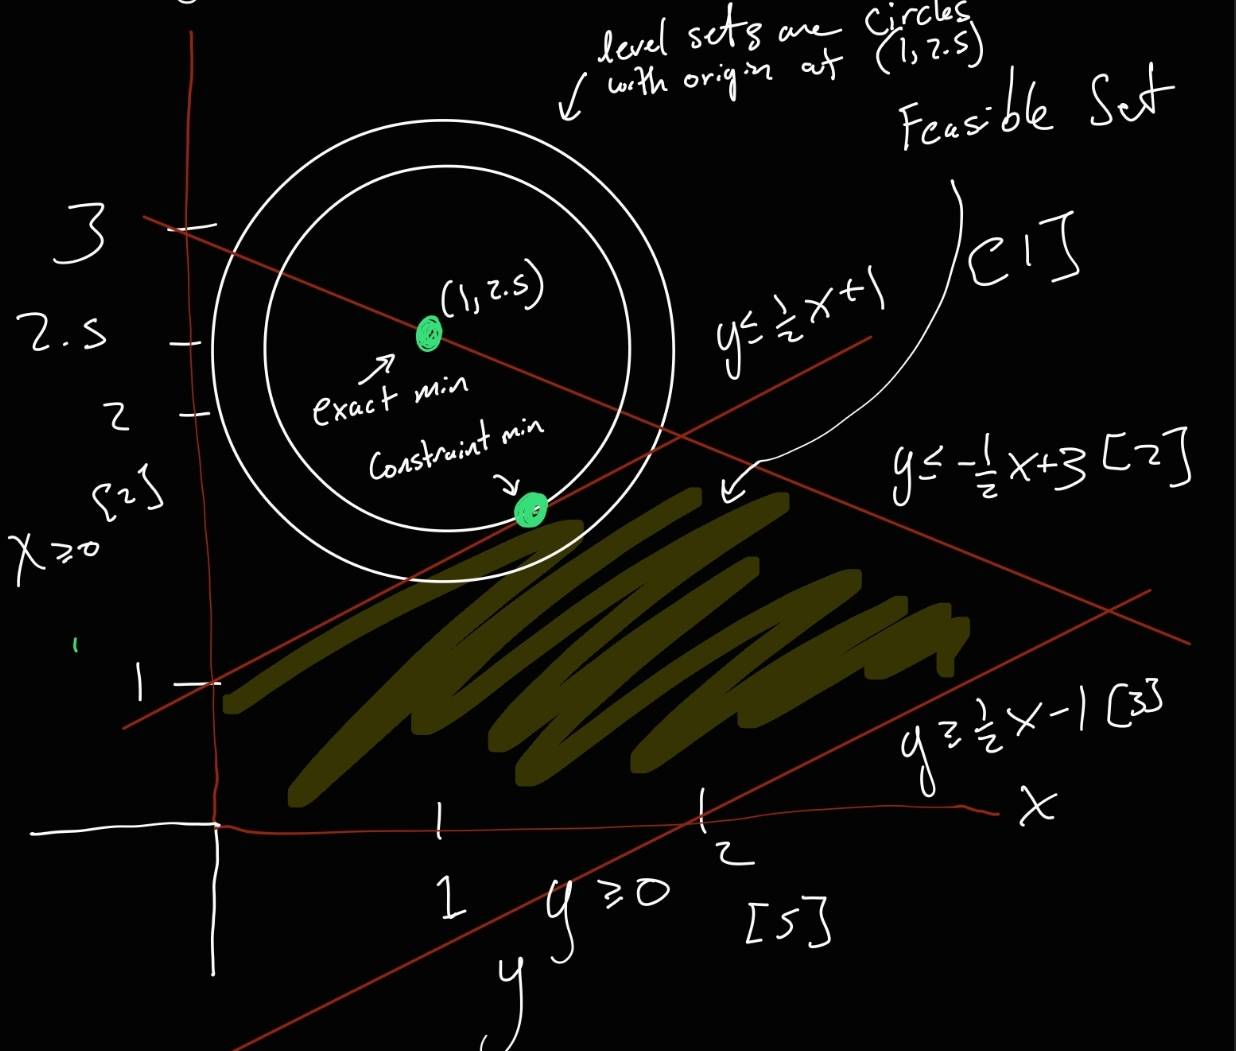
\includegraphics[width=0.6\textwidth,height=\textwidth,keepaspectratio]{plot.jpg}
    \caption{Plot of the quadratic problem (6)-(11). The level sets are shown in white, the constraint functions in red, the feasible set in yellow, and the solutions in green.}
    \label{fig}
\end{figure}
Consider the quadratic program with inequality constraints given by (6)-(10).
\begin{enumerate}
    \item [(a)]
    To plot the level sets of the objective function given in Eq. (6), we notice that these are circles with origin at $(1,2.5)$. Next, we can rewrite the constraints [1]-[3] to get
    \begin{align*}
        &[1] \quad y \leq \frac{1}{2}x + 1,\\
        &[2] \quad y \leq -\frac{1}{2}x + 3,\\
        &[3] \quad y \leq \frac{1}{2}-1.
    \end{align*}
    Plotting these we get Figure \ref{fig} where we can see the level sets and the feasible set.

    \item [(b)]
    Observing Figure \ref{fig}, we notice that the true minimum of $f(x,y)$ occurs at $(1,2.5)$. Thus we can see that the constrained minimum occurs when the level set of $f(x,y)$ intersects constraint [1]. Using that $y = \frac{1}{2}x + 1$, we get
    \begin{equation*}
        f(x) = (x-1)^2 + \paren{\frac{1}{2}x - \frac{3}{2}}^2.
    \end{equation*}
    Now we can take the derivative and find the minimum to get
    \begin{equation*}
        f'(x) = 2(x-1) + \paren{\frac{1}{2}x - \frac{3}{2}} = \frac{5}{2}x - \frac{7}{2} = 0 \iff x = \frac{7}{5}.
    \end{equation*}
    Therefore we find that the solution to (6)-(11) is given by $\paren{\frac{7}{5},\frac{17}{10}}$.
    
    
    \item [(c)]
    To apply the active-step method to this problem, let's rewrite the problem as
    \begin{align*}
        f(v) &= \frac{1}{2} v^\top G v + c^\top v \to \min ~\text{subject to}\\
        A_\mathcal{W} v &= b_\mathcal{W}, 
    \end{align*}
    where $v = (x,y)^\top$ and $\mathcal{W}$ is the current set of active constraints. Now by expanding 
    \begin{equation*}
        f(x,y) = (x - 1)^2 + (y - 2.5)^2 =  x^2 + y^2 - 2x - 5y + 1+ \frac{25}{4},
    \end{equation*}
    we find that the quadratic term is $x^2 + y^2$ and the linear part is $-2x - 5y$ and thus 
    \begin{equation*}
        G = \begin{pmatrix}
            2 & 0 \\ 0 & 2
        \end{pmatrix} \and c = \begin{pmatrix}
            -2 \\ -5
        \end{pmatrix}.
    \end{equation*}
    Suppose the initial point is $v_1 = (2,0)$. Then the active set of constraints is $\mathcal{W} = \brac{3,5}$. Thus we get
    \begin{equation*}
        A = \begin{pmatrix}
            -1 & 2 \\ 0 & 1
        \end{pmatrix} \and b =\begin{pmatrix}
            2 \\ 0
        \end{pmatrix}.
    \end{equation*}
    Finally, notice that the gradient is given by
    \begin{equation*}
        \nabla f(x_k,y_k) = (2x-2,2y-5)^\top,
    \end{equation*}
    so $\nabla f(v_1) = (2,-5)^\top$. Therefore KKT system on the first iteration is given by
    \begin{equation*}
        \begin{pmatrix}
            2 & 0 & -1 & 0\\
            0 & 2 & 2 & 1\\
            -1 & 2 & 0 & 0\\
            0 & 1 & 0 & 0\\
        \end{pmatrix}\begin{pmatrix}
            -p_{1_x}\\-p_{1_y}\\\lambda_{1_x}\\\lambda_{1_y}
        \end{pmatrix} = \begin{pmatrix}
            2 \\ -5 \\ 0 \\ 0
        \end{pmatrix}.
    \end{equation*}
    Now let's solve the KKT system for $p_1$ and $\lambda_1$. Observe that
    \begin{align*}
        \begin{pmatrix}
            2 & 0 & -1 & 0\\
            0 & 2 & 2 & 1\\
            -1 & 2 & 0 & 0\\
            0 & 1 & 0 & 0\\
        \end{pmatrix}\begin{pmatrix}
            -p_{1_x}\\-p_{1_y}\\\lambda_{1_x}\\\lambda_{1_y}
        \end{pmatrix} = \begin{pmatrix}
            -2p_{1_x} - \lambda_{1_x}\\ 2\lambda_{1_x} + \lambda_{1_y} - 2 p_{1_y}\\ p_{1_x} - 2 p_{1_y} \\ - p_{1_y}
        \end{pmatrix} = \begin{pmatrix}
            2 \\ -5 \\ 0 \\ 0
        \end{pmatrix}
    \end{align*}
    and solving the linear system of equations yields
    \begin{equation*}
        p_1 = \begin{pmatrix}
            0 \\ 0
        \end{pmatrix} \and \lambda_1 = \begin{pmatrix}
            -2 \\ -1
        \end{pmatrix},
    \end{equation*}
    since both components of $\lambda_1$ are negative, we remove both of the constraints and set $v_2 = v_1 + p_1$.

    On the second iteration, the iterate is $v_2 = (2,0)$ and the active set is $\mathcal{W} = \emptyset$. We compute that $\nabla f(v_2) = (2,-5)^\top$. Therefore the KKT system on the second iteration is given by
    \begin{equation*}
        \begin{pmatrix}
            2 & 0 \\
            0 & 2 \\
        \end{pmatrix}\begin{pmatrix}
            -p_{2_x}\\-p_{2_y}
        \end{pmatrix} = \begin{pmatrix}
            -2p_{2_x}\\-2p_{2_y}
        \end{pmatrix}= \begin{pmatrix}
            2 \\ -5
        \end{pmatrix}.
    \end{equation*}
    Solving this system gives
    \begin{equation*}
        p_2 = \begin{pmatrix}
            -1 \\ 5/2
        \end{pmatrix}.
    \end{equation*}
    Now notice that $v_2 + p_2$ is out of the feasible set, so let's find the step size given by
    \begin{equation*}
        \alpha_2 = \min\brac{1,\min_{i\not\in\mathcal{W},a_i^\top p_2}\frac{b_i - a_i^\top p_2}{a_i p_2}} = \min\brac{1,\frac{b_1 - a_1^\top p_2}{a_1 p_2}} = \min \brac{1, \frac{2}{3}} = \frac{2}{3},
    \end{equation*} 
    and thus we update $v_3 = v_2 + \alpha_2 p_2$.

    On the third iteration, the iterate is $v_3 = (4/3,5/3)$ and so the first constraint is active meaning that $\mathcal{W} = \brac{1}$. Then $A = (1, -2)^\top$ and $\nabla f(v_3) = (2/3, -5/3)$. Therefore the KKT system is given by
    \begin{equation*}
        \begin{pmatrix}
            2 & 0 & 1\\
            0 & 2 & -2\\
            1 & -2 & 0\\
        \end{pmatrix}\begin{pmatrix}
            p_{3_x}\\p_{3_y}\\\lambda_3
        \end{pmatrix}=\begin{pmatrix}
            2/3\\-5/3\\0
        \end{pmatrix}
    \end{equation*}
    Solving this system gives
    \begin{equation*}
        p_3 = \begin{pmatrix}
            1/15 \\ 1/30
        \end{pmatrix} \and \lambda_3 = 4/5,
    \end{equation*}
    and thus we update $v_4 = v_3 + p_3$.

    On the fourth iteration, the iterate $v_4 = (7/5,17/10)$ and so the first constraint us active meaning that $\mathcal{W} = \brac{1}$. Then $A = (1, -2)^\top$ and $\nabla f(v_4) = (4/5, -8/5)$. Therefore the KKT system is given by
    \begin{equation*}
        \begin{pmatrix}
            2 & 0 & 1\\
            0 & 2 & -2\\
            1 & -2 & 0\\
        \end{pmatrix}\begin{pmatrix}
            p_{4_x}\\p_{4_y}\\\lambda_4
        \end{pmatrix}=\begin{pmatrix}
            4/5\\-8/5\\0
        \end{pmatrix}
    \end{equation*}
    Solving this system gives
    \begin{equation*}
        p_4 = \begin{pmatrix}
            0 \\ 0
        \end{pmatrix} \and \lambda_4 = 4/5.
    \end{equation*}
    Since $p_4 = \vec{0}$ and $\lambda_4 > 0$, we have found the solution to be $(7/5,17/10)$ which corresponds with the solution, we found in part (b). The iterates can be seen in Figure \ref{fig22}.

    
    
    
    
    \begin{figure}
        \centering
        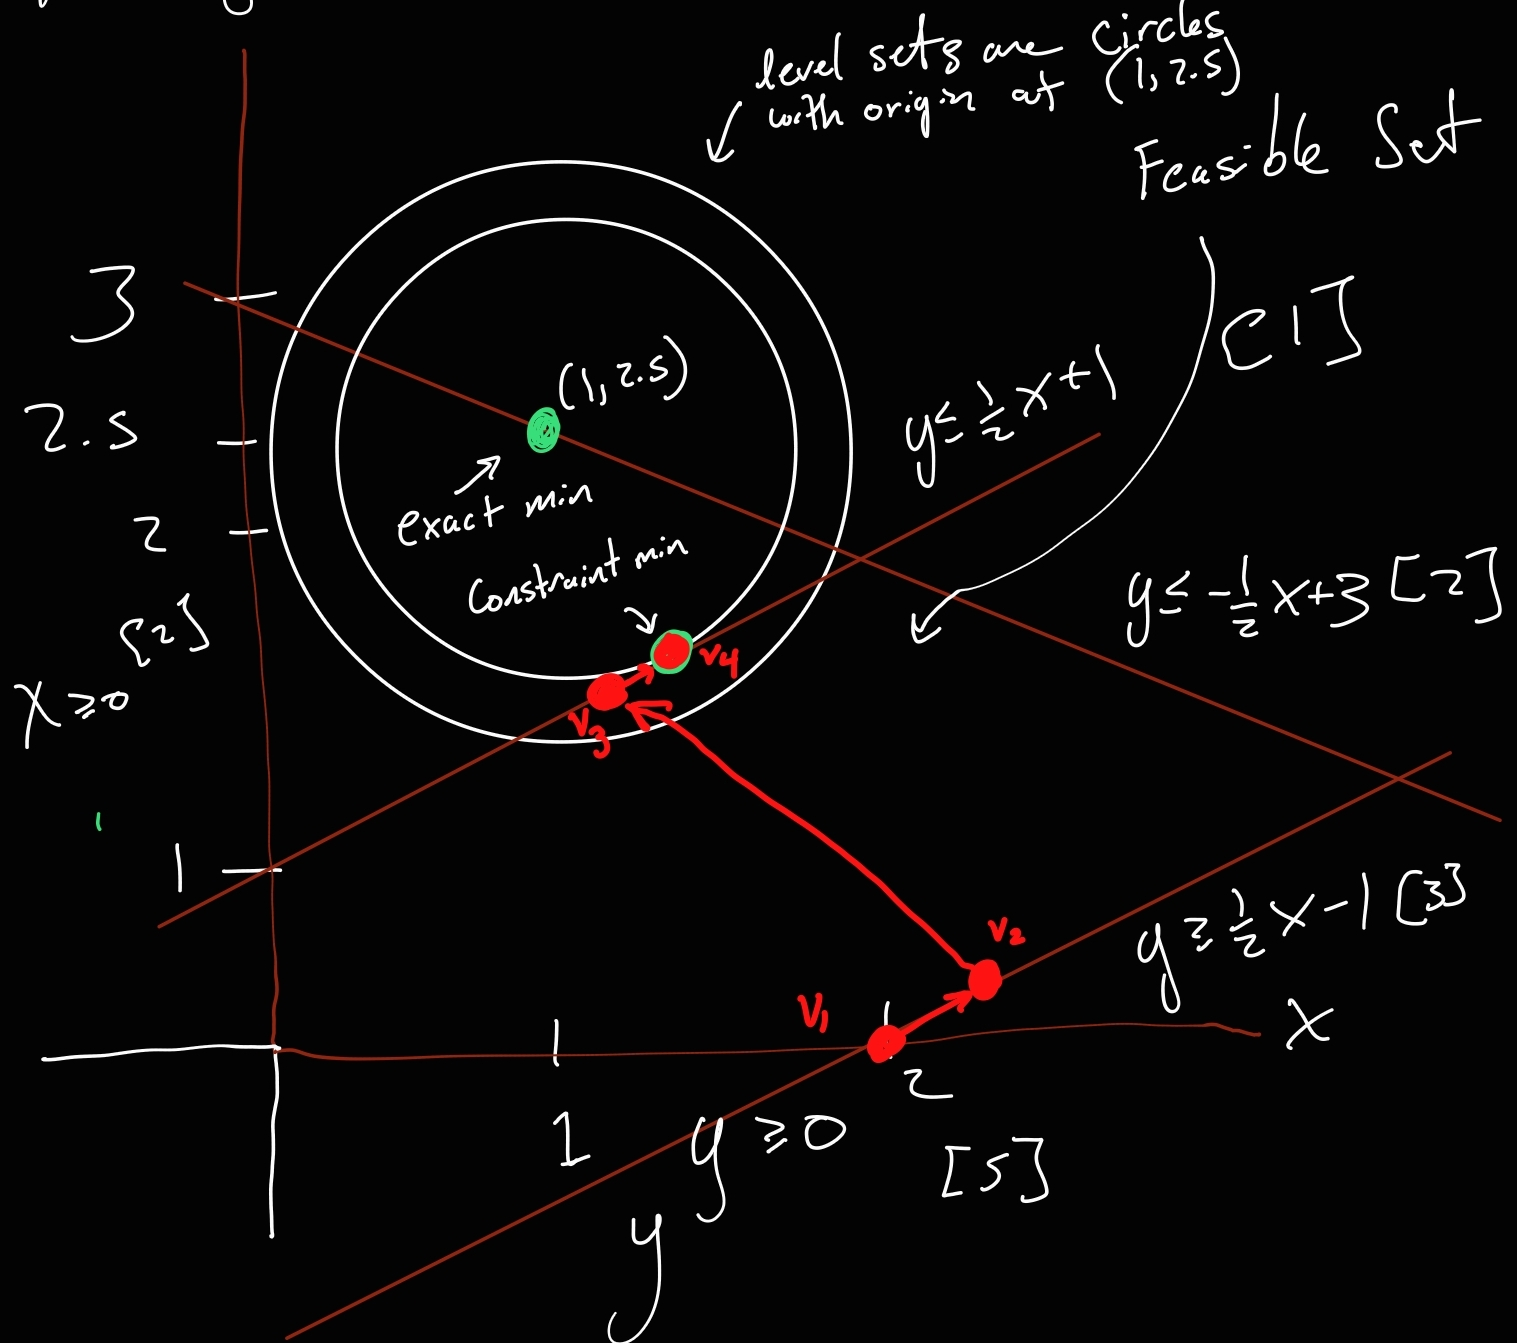
\includegraphics[width=0.5\textwidth,height=\textwidth,keepaspectratio]{plokt2.jpg}
        \caption{The iterates of the KKT active-step method can be seen in bright red.}
        \label{fig22}
    \end{figure}
    
    
    
    
    
    
    
    
    
    
    
    
    
    
    
    
    % , we need to modify the active set. Let's remove constraint [5] from the set. Now we update $v_2 = v_1 + p_1$. On the second iteration, the iterate is $v_2 = (2,0)$ and the active set is $\mathcal{W} = \brac{1}$. Thus $A = (-1,2)$ and $\nabla f(v_2) = (2,-5)^\top$. Therefore, the KKT system is given by
    % \begin{equation*}
    %     \begin{pmatrix}
    %         2 & 0 & -1\\
    %         0 & 2 & 2\\
    %         -1 & 2 & 0
    %     \end{pmatrix}\begin{pmatrix}
    %         -p_{2_x}\\-p_{2_y}\\\lambda_{2}
    %     \end{pmatrix} = \begin{pmatrix}
    %         -2p_{2_x} - \lambda_2 \\ 2\lambda_2 - 2 p_{2_y} \\ p_{2_x}-2p_{2_y}
    %     \end{pmatrix}= \begin{pmatrix}
    %         2 \\ -5 \\ 0
    %     \end{pmatrix}.
    % \end{equation*}
    % Solving this system gives
    % \begin{equation*}
    %     p_2 = \begin{pmatrix}
    %         1/5 \\ 1/10
    %     \end{pmatrix} \and \lambda_2 = -\frac{12}{5}.
    % \end{equation*}
    % Thus we update $v_3 = v_2 + p_2$. On the third iteration, the iterate is $v_3 = (11/5,1/10)^\top$, meaning that the constraint [3] is active, thus $\mathcal{W} = \brac{3}$. Then $A = (-1,2)$ and $\nabla f(v_3) = (12/5, -24/5)^\top$. Therefore, the KKT system is given by
    % \begin{equation*}
    %     \begin{pmatrix}
    %         2 & 0 & -1\\
    %         0 & 2 & 2\\
    %         -1 & 2 & 0
    %     \end{pmatrix}\begin{pmatrix}
    %         -p_{3_x}\\-p_{3_y}\\\lambda_{3}
    %     \end{pmatrix} = \begin{pmatrix}
    %         -2p_{3_x} - \lambda_3 \\ 2\lambda_3 - 2 p_{3_y} \\ p_{3_x}-2p_{3_y}
    %     \end{pmatrix}= \begin{pmatrix}
    %         12/5 \\ -24/5 \\ 0
    %     \end{pmatrix}.
    % \end{equation*}
    % Solving this system gives
    % \begin{equation*}
    %     p_3 = \begin{pmatrix}
    %         0 \\ 0
    %     \end{pmatrix} \and \lambda_3 = -\frac{12}{5}.
    % \end{equation*}
    % Thus we update $v_4 = v_3 + p_3$ and since $\lambda_3 < 0$ we remove constraint [1] from the set. On the fourth iteration, the iterate is $v_4 = (11/5,1/10)^\top$ with no active constraints. Therefore, the KKT system is given by
    % \begin{equation*}
    %     \begin{pmatrix}
    %         2 & 0 \\
    %         0 & 2 \\
    %     \end{pmatrix}\begin{pmatrix}
    %         -p_{4_x}\\-p_{4_y}
    %     \end{pmatrix} = \begin{pmatrix}
    %         -2p_{4_x}\\-2p_{4_y}
    %     \end{pmatrix}= \begin{pmatrix}
    %         12/5 \\ -24/5
    %     \end{pmatrix}.
    % \end{equation*}
    % Solving this system gives
    % \begin{equation*}
    %     p_4 = \begin{pmatrix}
    %         -6/5 \\ 12/5
    %     \end{pmatrix}.
    % \end{equation*}
    % \begin{figure}
    %     \centering
    %     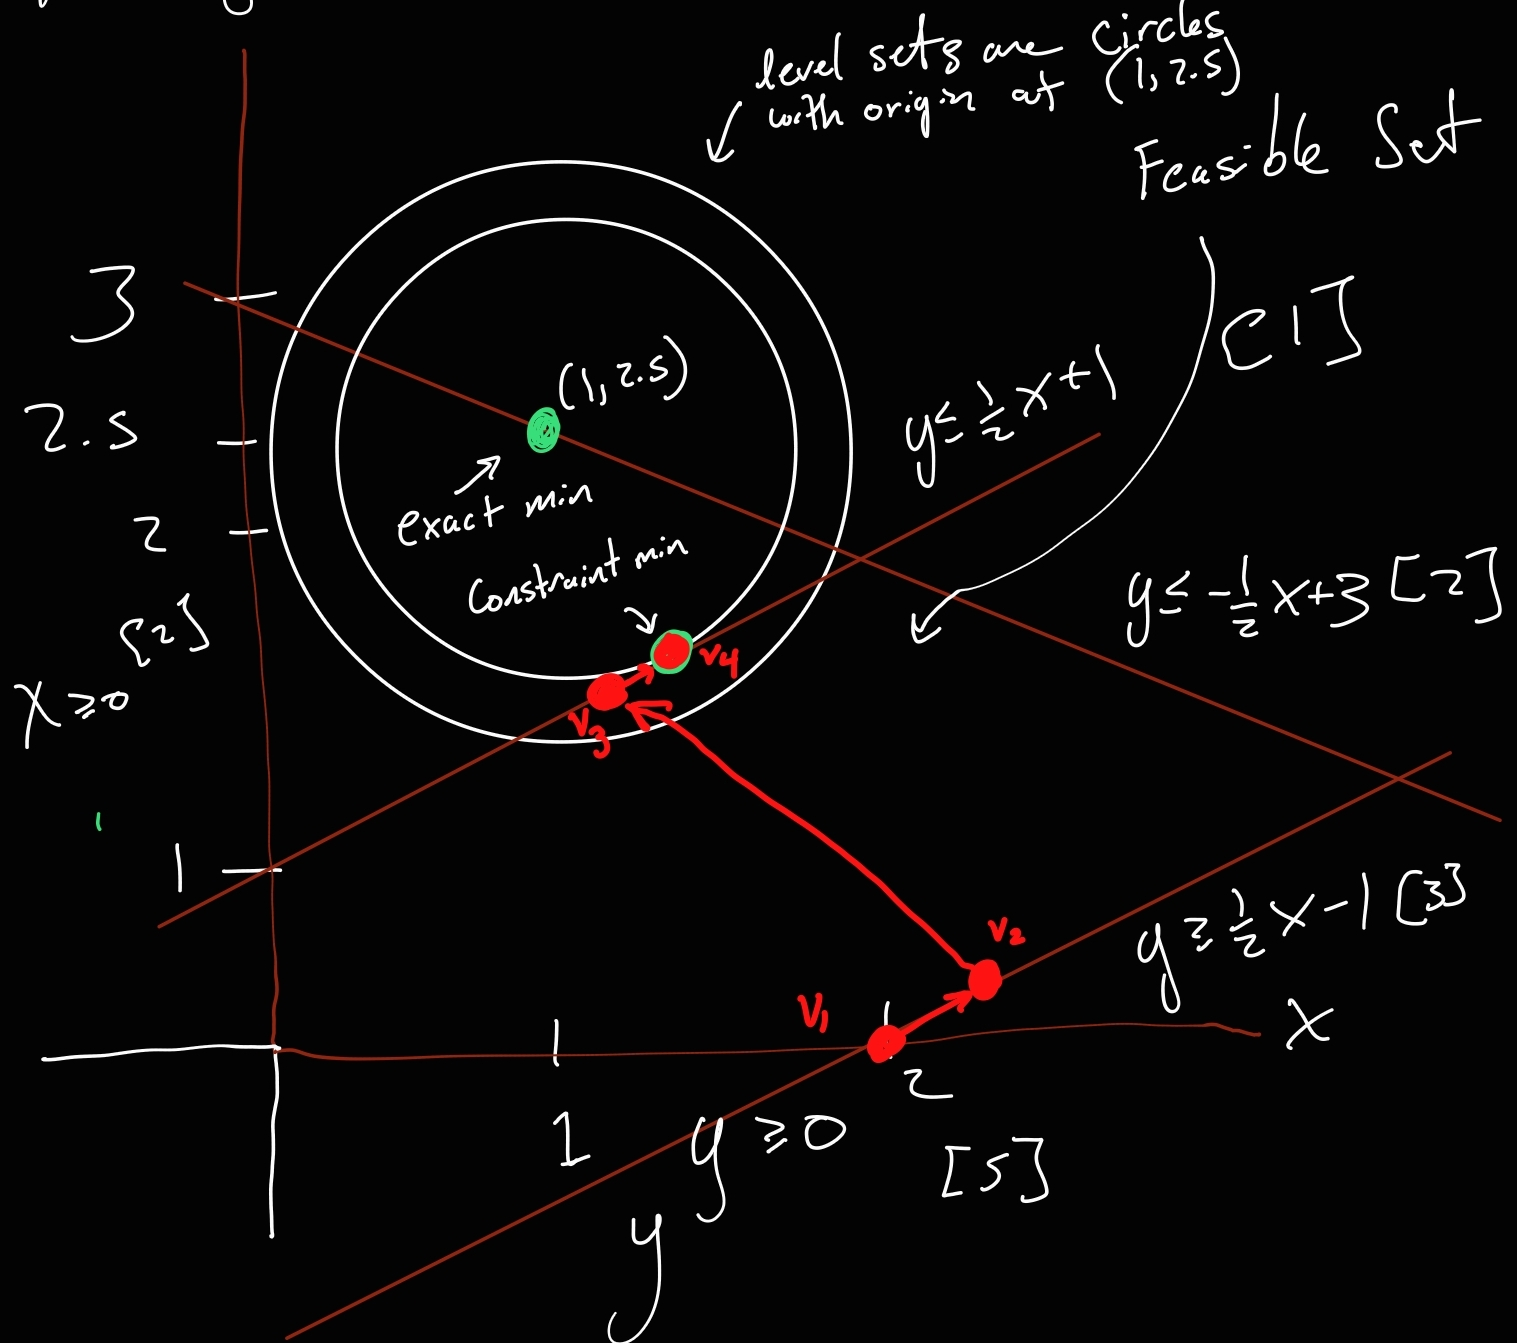
\includegraphics[width=0.5\textwidth,height=\textwidth,keepaspectratio]{plokt2.jpg}
    %     \caption{The iterates of the KKT active-step method can be seen in bright red.}
    %     \label{fig22}
    % \end{figure}
    % Notice that the update $v_4 + p_4 = (1,5/2)$ is outside the feasible set so we compute
    % \begin{equation*}
    %     \alpha = \min\brac{1,\min_{i\not\in\mathcal{W}}\frac{b_i - a_i^\top p_4}{a_i p_4}} = \min\brac{1,\frac{b_2 - a_2^\top p_4}{a_i p_4}} = \min\brac{1,\frac{2}{3}} = \frac{2}{3}.
    % \end{equation*}
    % Then $v_5 = v_4 + \alpha p_4.$ Finally, on iteration five, the iterate is $(7/5,17/10)$ meaning that the first constraint is active and thus $\mathcal{W} = \brac{1}$. Then $a=(1,-2)$ and $\nabla(v_5) = (8/10,-16/10)^\top$. Therefore, the KKT system is given by
    % \begin{equation*}
    %     \begin{pmatrix}
    %         2 & 0 & 1\\
    %         0 & 2 & -2\\
    %         1 & -2 & 0
    %     \end{pmatrix}\begin{pmatrix}
    %         -p_{5_x}\\-p_{5_y}\\\lambda_{5}
    %     \end{pmatrix} =\begin{pmatrix}
    %         8/10 \\ -16/10 \\ 0
    %     \end{pmatrix}.
    % \end{equation*}
    % Solving this system gives
    % \begin{equation*}
    %     p_5 = \begin{pmatrix}
    %         0 \\ 0
    %     \end{pmatrix} \and \lambda_5 = 8/10.
    % \end{equation*}
    % Since $p_5 = \vec{0}$ and $\lambda_5 > 0$ we have found the solution to be $(7/5,17/10)$ which corresponds with the solution, we found in part (b). The iterates can be seen in Figure \ref{fig22}.





\end{enumerate}

\end{proof}
\end{problem}


\end{document}